\documentclass[11pt]{article}
\usepackage[margin=0.7in]{geometry}
\usepackage{graphicx}
\usepackage[hidelinks]{hyperref}
\pagestyle{plain}
\begin{document}
\section*{Graphical revision: Figure 2(d)}
The original and revised panels use the same curves, gate, probe marks, event
window and axis limits. The added annotation identifies the shared score spike
13.5 hours after onset, after the shaded disturbance ends at 12 hours. The spike
also occurs in the paired unmodified background. Figures 1, 3 and 4 are unchanged.

\noindent\textbf{Before: preserved comparison baseline}
\begin{center}
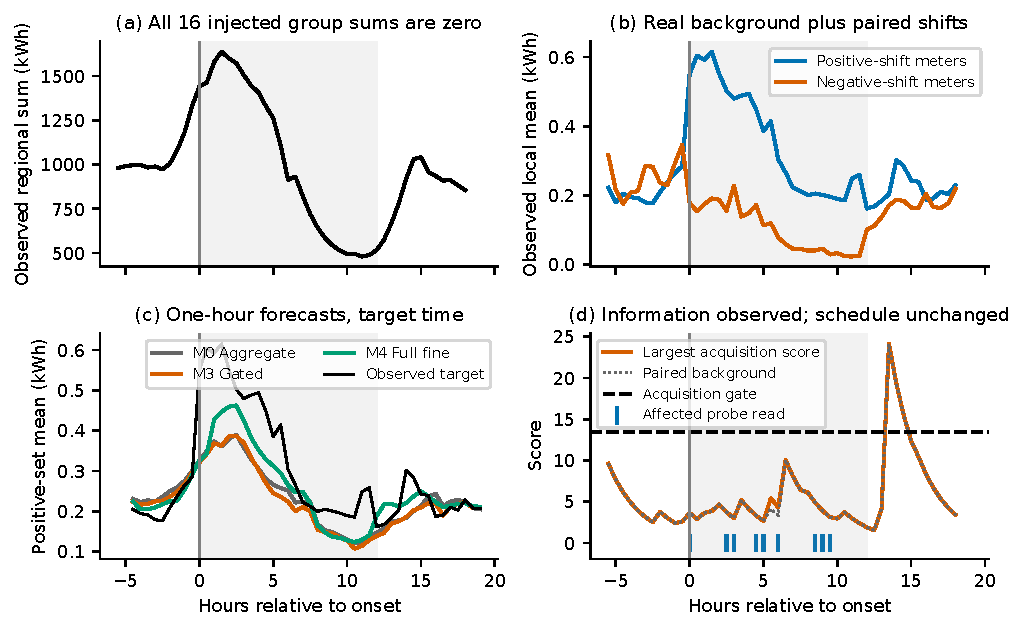
\includegraphics[width=.90\textwidth]{baseline/manuscript/figures/transparent_episode.pdf}
\end{center}
\newpage
\noindent\textbf{After: Figure 2(d) annotated}
\begin{center}
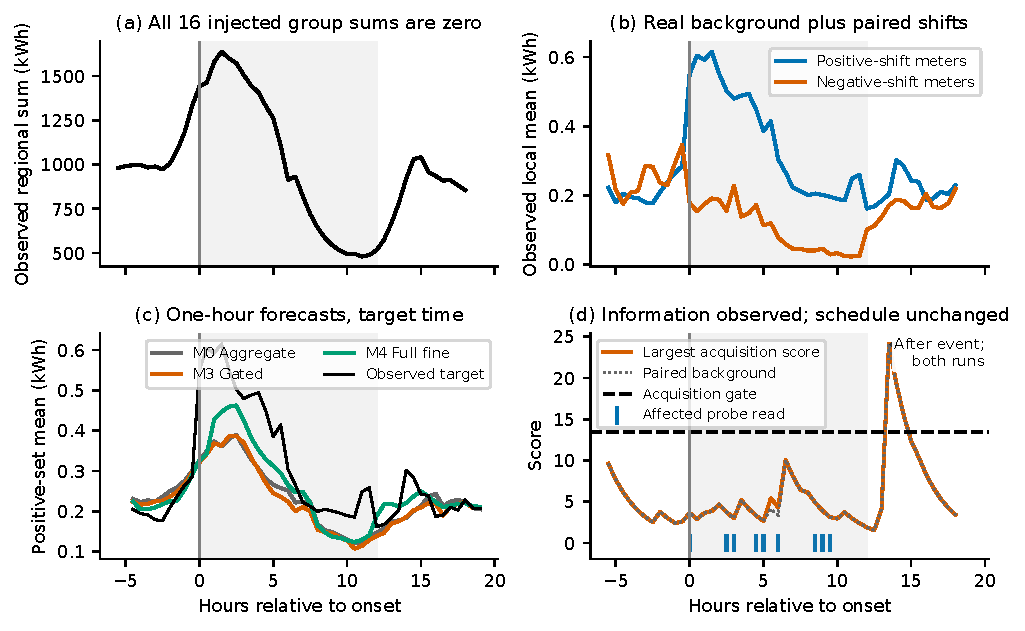
\includegraphics[width=.95\textwidth]{figures/transparent_episode.pdf}
\end{center}
\noindent This annotation adds no experimental result. The plotted values and
input hashes are recorded in \path{analysis/figure_annotation.json}.
The separate \path{figures/alarm_sweep.pdf} is new technical-note material,
reproduced by \path{scripts/analyze_alarm_sweep.py}; its matched-rate table
appears in the revised paper.
\end{document}
